d\chapter{Introduction}
\label{sec:intro}

Why does a person like a particular song? What are the inherent aspects of a song that pleases a person's musical taste? Is it the complexity of a song, the beat the song or just a particular melodic pattern ? More so if a person likes a song, can we predict if he/she will like a similar song? \\\\
Music has been created since the dawn of civilization and these questions have plagued mankind just as long. In response to this, man has created elaborate systems of formal study for music and classification techniques in almost every ethnic community since antiquity. Two notable examples are the western system of solfege and classical music theory and the Indian system of raagas. These elaborate systems are based on very simple fundamental building blocks of melody and harmony and simple rules that govern the interplay of these building blocks. However very complex pieces of music can be created with these simple rules depending on the skill and virtuosity of artists. Composers use these rules and concepts to create novel music for mass consumption. \\\\
In the modern era industry and academia have attempted to address the problem of music recommendation and music classification. The industry has predominantly favored approaches that look at user preferences and history. For example Amazon Music recommendation works on users shopping history. Pandora on the other hand hires an army of musicologists to ascertain how a song is similar to another song and creates software that leverages this adhoc generated data. These approaches are either expensive in the human labor needed or in the amount of data processed that is input from a large number of users. More recently, companies like Echo Nest has extensively extracted features from music sources and mined cultural information on the web but leave it at consumers how best to leverage the data. Hence symbolic MIR is not traditionally used in industry and music theory is an after thought. \\\\
Academia on the other hand attempts to solve very particular problems in MIR. Typical examples would be cover song detection, processing information via signal processing, audio feature extraction, optical music recognition etc. In most cases the applications are of a very specific domain and does not fully scale with bulk music data. Generic frameworks like the jMIR (which also happens to be a major inspiration for modulo7) suite for automatic music classification exists, which is meant to facilitate research in MIR with a machine learning focus. However academia is disconnected with industry and no full scale MIR engines can satisfy the scale of industry applications. \\\\
This work is attempt to bridge both communities. Modulo7 is a full stack deployment, providing both a server architecture and a sql like client to query based on music theory criteria.
\chapter{Server side architecture}
Modulo7 is designed with the purpose of scalability. A block diagram of the components of the server side architecture is presented below :-
\begin{enumerate}
\item Source Converter : Converts music sources (e.g. music XML, midi etc) into modulo7's binary representation.
\item Music Theory Models : The model is a description of music theoretic criteria that can be applied on top of song. Examples would be melodic contour, tonal histogram etc. 
\item Distributed Storage Mechanism : The modulo7 internal representation is 
\end{enumerate}

\begin{figure}[t]
\centering
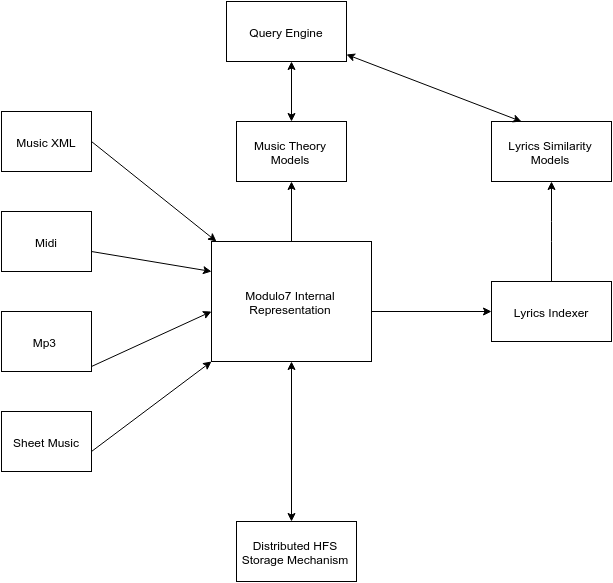
\includegraphics[width=\textwidth]{Modulo7ServerDesign.png}
\makeatletter
\let\@currsize\normalsize
\caption{Modulo7 server architectural design}
\label{fig:figure}
\end{figure}

\chapter{Progress Done}
